\chapter{機器學習的訓練與模擬控制結果}
\section{訓練模型的基礎概念}
 訓練模型的原型是實體冰球機的機電系統,由於要訓練強化學習,所以需要將模型簡化至最簡潔的方式進行訓練,並取Open AI Gym的環境當作最簡化的訓練模型。由於強化學習是一種最佳化控制的方式,因此將Gym的Pong畫面當作輸入,輸出為擊錘移動方向,藉由調整當中的權重、偏差等參數,將參數調配到最優狀態。將可行的訓練方式套用到CoppeliaSim進行虛擬環境的訓練,並且可將訓練結果套用到實機進行運用。\\
\section{訓練模型的選用}
 利用Gym的環境訓練機器學習,以測試學習率、神經網路隱藏層的神經元個數、機器學習的啟動函數類型、訓練時影像大小等幾項參數與訓結果之間的關聯性,選用pyhton語言進行配置。剛開始我們運用Pygame模組來撰寫pong game的訓練環境,開始學習並了解Pygame的一些運用,嘗試建構出pong game場景(圖.\ref{fig.pong_pygame}),在基本功能編寫告一段落後,測試程式漏洞,發現對打時特定角度碰撞,球會超過擊錘的碰撞感測,導致出現球擊穿擊錘的現象。為了解決Pygame碰撞問題,做了幾種嘗試:修改Pygame的碰撞定義,更換碰撞感測的感測方式,問題依舊沒有顯著的改善,若增加過多的碰撞偵測點則會造成後續機器學習訓練時的運算負荷;另一種方法則是搭配pymunk的物理引擎模組使用(圖.\ref{fig.airhockey_pymunk}),使環境更符合實際物理現象,可加入碰撞、摩擦、力量大小、速度大小等可以個別設定和調用。當環境有了物理接下來就需要加入訓練所需的功能,如:訓練時的場景的即時影像畫面、即時獎勵回傳、該局結束時的場景重設和分數重置等功能。此時找到了Open AI Gym模組。\\
\begin{figure}[hbt!]
\begin{center}
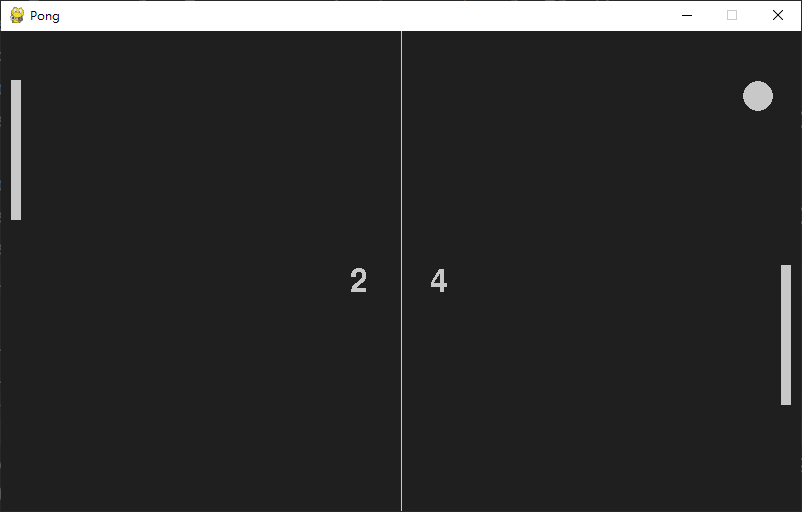
\includegraphics[width=12cm]{pong_pygame}
\caption{\Large Pygame模組編寫}
\label{fig.pong_pygame}
\end{center}
\end{figure}

\begin{figure}[hbt!]
\begin{center}
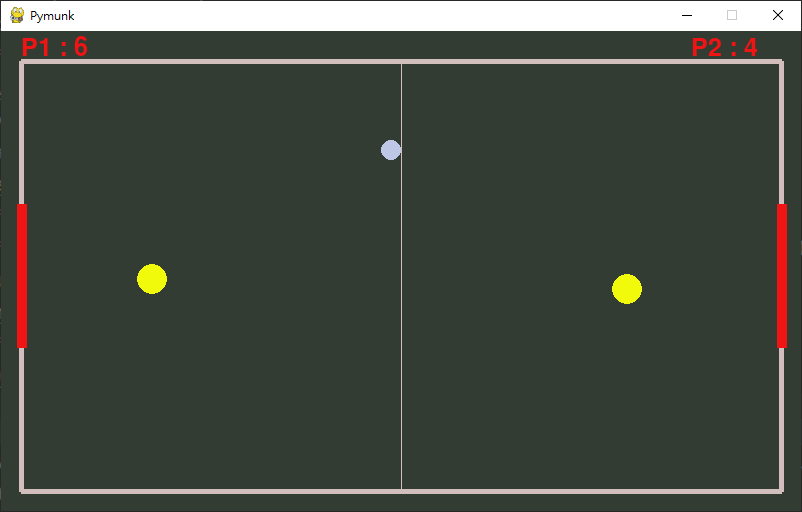
\includegraphics[width=12cm]{airhockey_pymunk}
\caption{\Large Pymunk模組編寫}
\label{fig.airhockey_pymunk}
\end{center}
\end{figure}
 \newpage %圖片空隙勿刪
 Open AI Gym裡面有十幾種訓練模型的環境,提供機器學習做訓練的環境。由於我們的訓練模型是pong game,在Gym模組裡面剛好有訓練模型,因此使用Gym模組相對於使用Pygame和pymunk的搭配來的方便,而且後續要在CoppeliaSim模擬環境模擬時也有套件可搭配使用,可簡化功能和訓練時所需的環境模型和訓練功能的程式編寫,另一方面自寫場景需要測試場景的漏洞,使用Gym可以節省檢查場景漏洞和修正的時間。\\
\section{訓練程式的運作}
 由於機器學習和影像處理需要大量的運算矩陣運算,因此如果只單獨透過Python本身運算比編譯語言執行的速度來的慢,所以使用Numpy程式庫來解決在Python環境矩陣運算速度慢的問題,以提升訓練機器學習時的運算效率。pickle是Python內部的序列化方式,主要是當機器學習訓練時可能因為一些原因需要暫時停止訓練,但為了讓已經停下的訓練再次重啟就需要透過pickle序列化的方式,將暫停前的訓練權重值透過pickle將其記錄下來,當訓練再次重啟時就可透過pickle.load讀取先前紀錄的pickle檔案就可回到當時暫停的狀態下繼續進行訓練。\\
 
 機器學習所運用的架構是強化學習並搭配神經網路來訓練機器學習,結合了強化學習不需要事先收集訓練資料、不需要特別教導,以及神經網路的非線性激活函數的計算和參數的記憶性。\\

\begin{figure}[hbt!]
\begin{center}
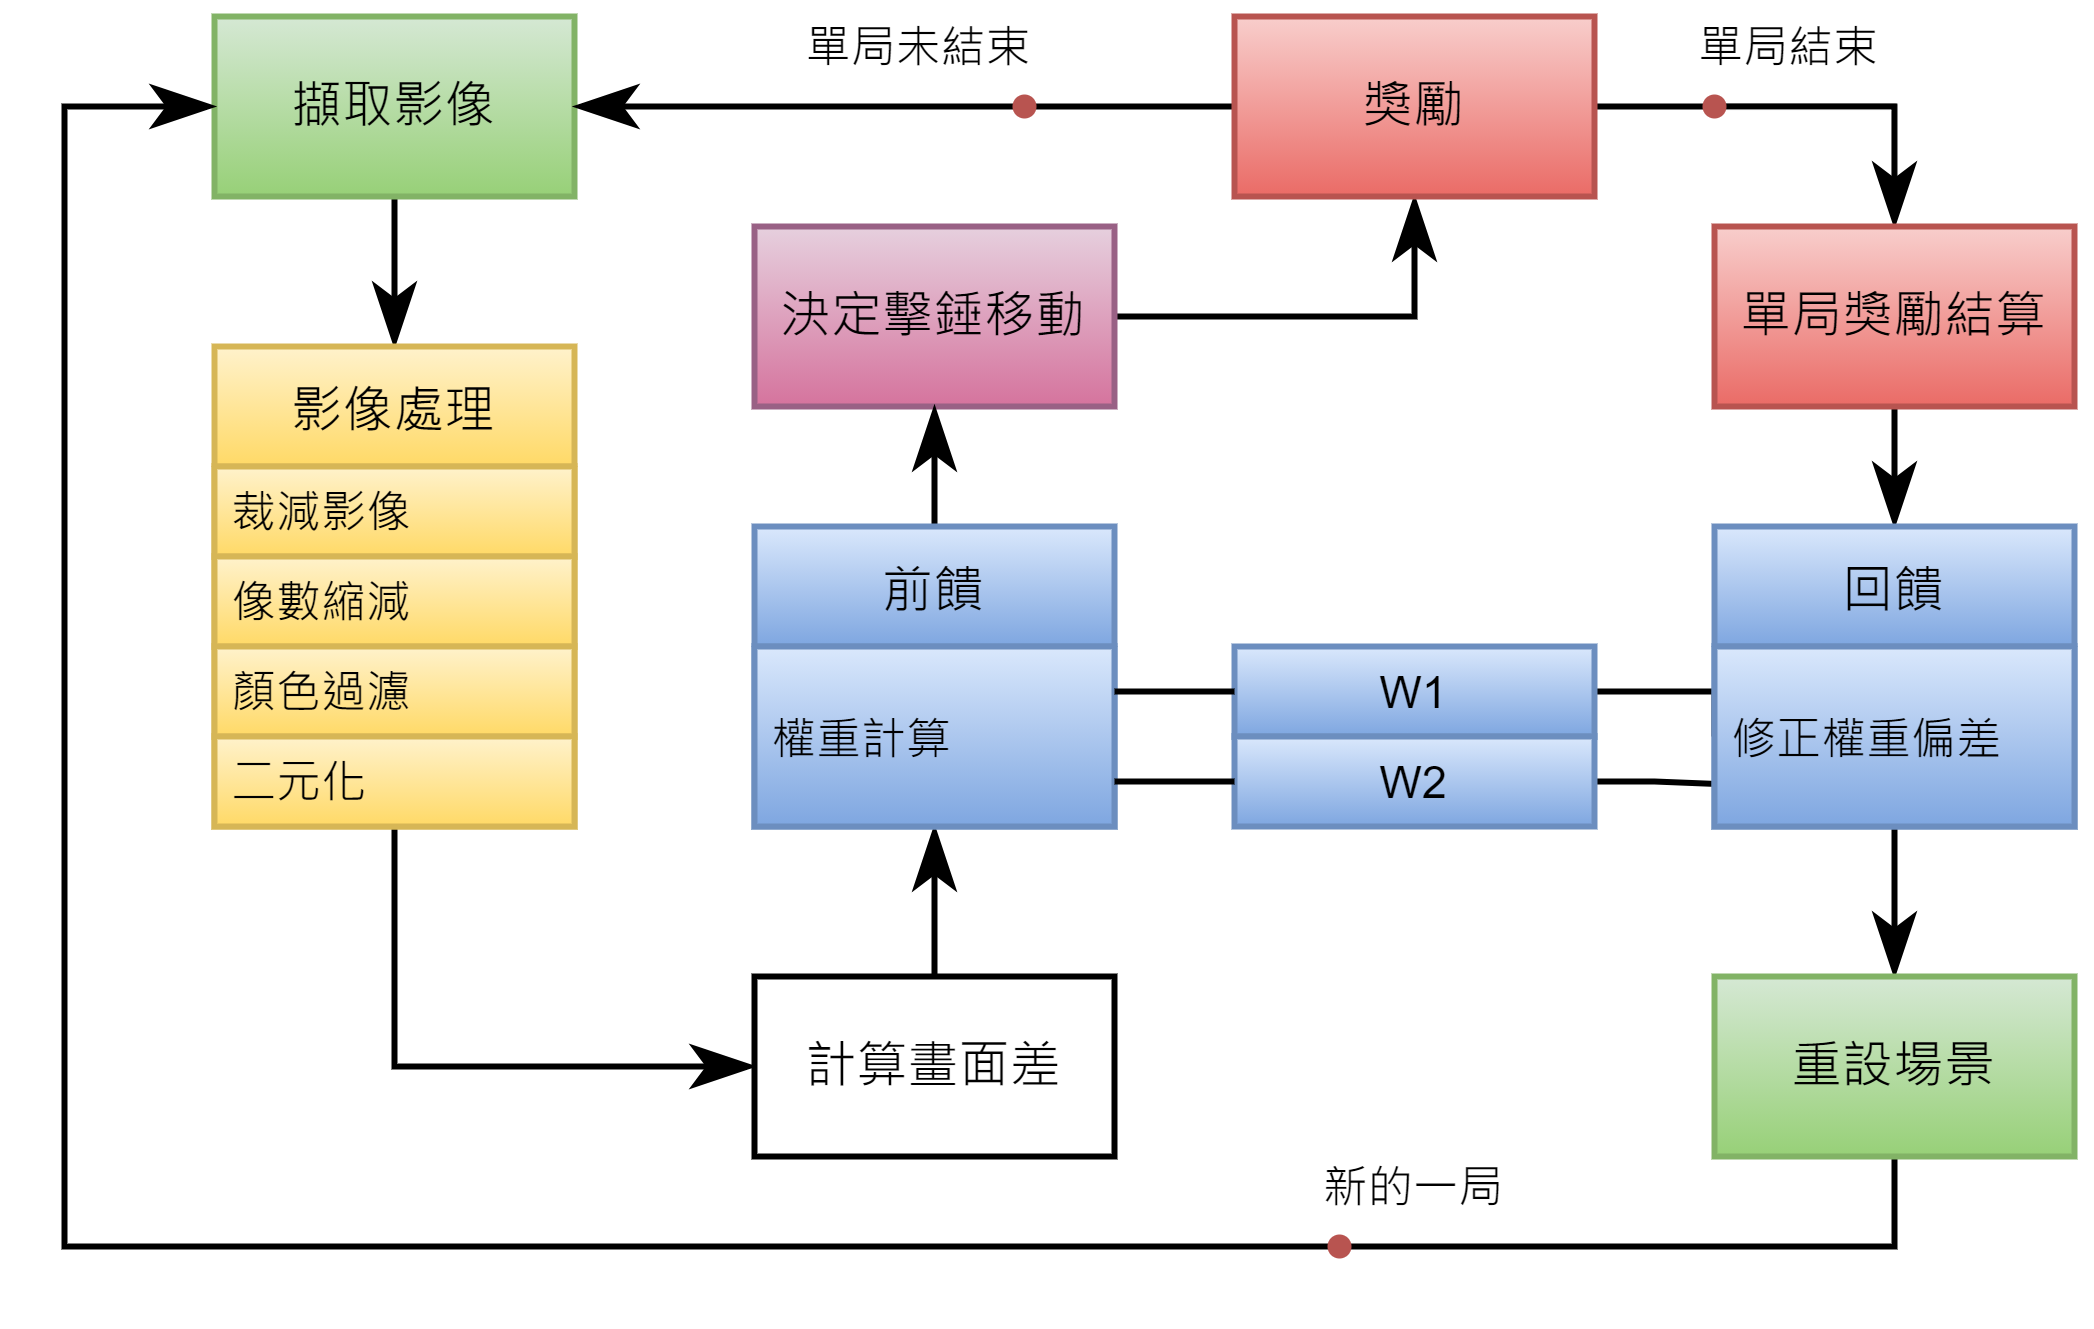
\includegraphics[width=15cm]{強化學習訓練流程}
\caption{\Large 強化學習訓練流程}
\label{fig.強化學習程式流程}
\end{center}
\end{figure}
%-----------------------------%

%=---------圖片空隙勿刪--------=%
%-----------------------------%
程式訓練流程(圖.\ref{fig.強化學習程式流程}):\\
 擷取影像,將影像裁剪至實際遊戲範圍,並簡化像素以利提高訓練時的計算速度,減少運算時的負擔,過濾顏色只保留球與擊錘,並把取到的影像二元化,取兩幀畫面進行比較,掌握球與擊錘間的相對位置(畫面差),透過前饋:計算球在環境的狀態及擊錘移動的決策,畫面差透過W1權重來計算球在環境的狀態,透過W2權重並經過啟動函數(activation function)得出擊錘移動的決策。透過產生隨機值的方式來與擊錘移動決策值進行比較,判定隨機值落在的區間來決定移動策略。計算discount reward及獎勵的加總。獎勵設定球若超過了對手,獎勵為+1;如果錯過球,則獎勵為-1;其餘狀態獎勵為0。\\

 在單局結束時,紀錄下該局累積下來的經驗,亦是紀錄該局所修正出來的參數而進行獎勵計算、log probability、RMSprop優化率減因子和反饋(back propagation),當訓練次數到達指定次數會以pickle做紀錄,存下的數據可再次導入模型進行實際運用,或是當程式中斷後可重新匯入進行訓練。比較持續訓練與中斷後重新匯入訓練的差異,測試算法版本為Pong2,MSE代表均方誤差值,pong2\_ r表示中斷後重新匯入的訓練數據,pong2與pong2\_ r標示個別表示該訓練每局分數的紀錄,pong2 MSE與pong2\_ r MSE標示個別表示該訓練均方誤差值紀錄(圖.\ref{fig.比較中斷數據}) \\
\begin{figure}[hbt!]
\begin{center}
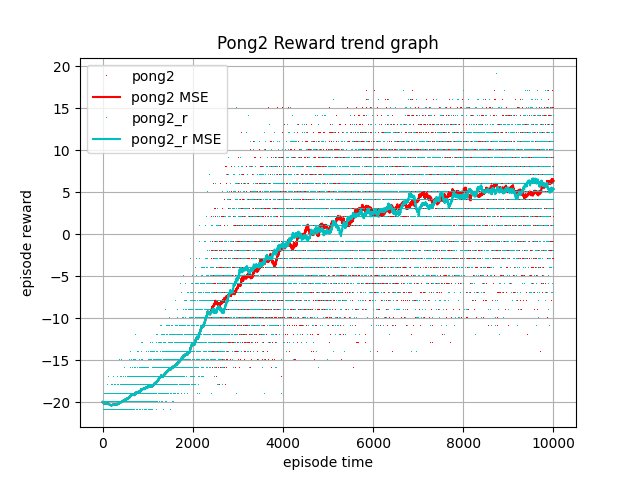
\includegraphics[width=15cm]{pong2_RvsNR}
\caption{\Large 比較中斷後訓練差異}
\label{fig.比較中斷數據}
\end{center}
\end{figure}

\section{訓練算法與參數比較}
 pong1版本是karpathy的pg\- pong.py的原始碼[\ref{R.pong1}],pong1.1原始碼則是schinger的pong\_ actor\- critic/pg\- pong\- ac.py[\ref{R.pong1.1}],pong1.2的是修改pong1的學習率參數從0.001調整到0.0001,並且將裁切後80*80的影像改成75*80。pong2將pong1的學習率保留不變,將啟動函數從sigmoid替換成softmax,並且將CPU運算換成GPU運算。下圖(圖.\ref{fig.比較中斷數據})為這幾個版本的訓練趨勢的紀錄提供做比較,訓練次數(圖.\ref{fig.比較中斷數據}之水平軸)為3000局做比較,小點為每局積分總和(圖.\ref{fig.比較中斷數據}之垂直軸),線條為累積積分的均方誤差值,積分計算-21分代表對面得21分,即機器訓練所得分數-對面所得分數。訓練存在隨機性(Stochastic),因此每次訓練所得趨勢會有所差異。
\begin{table}[hbt!]
\center\large
\setlength{\tabcolsep}{0.75cm}{
\begin{tabular}{|c|c|c|}
\hline  版本名稱 & 標示顏色 & 參考來源\\
\hline  pong1 &  紅色 & [\ref{R.pong1}]\\
\hline  pong1.1 &  藍色 & [\ref{R.pong1.1}]\\
\hline  pong1.2 &  橘色 & [\ref{R.pong1}]\\
\hline  pong2 & 綠色 & [\ref{R.pong1}] \\
\hline
\end{tabular}}
\caption{\Large 算法標示}
\end{table}

\begin{figure}[hbt!]
\begin{center}
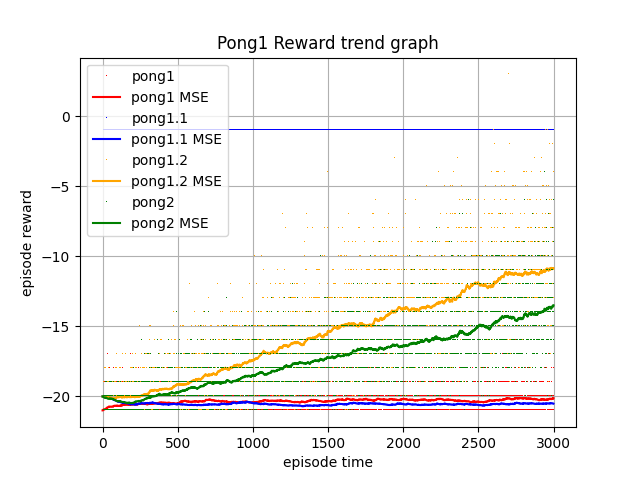
\includegraphics[width=15cm]{pong}
\caption{\Large 各算法差異}
\label{fig.比較中斷數據}
\end{center}
\end{figure}
觀察後得到,
 
\section{CoppeliaSim RemoteAPI}
在進行強化學習時主要是透過CoppeliaSim中的Remote API 函數來取得模擬場景中所需要的資訊,並在進行訓練後再回傳到CoppeloaSim做控制的動作。\\
\subsection{Remote API模組及動態連結函示庫}
在啟用RemoteAPI需要先準備以下三項模組和動態連結函示庫,並將此三項與預執行的程式放在同一目錄下:
\begin{itemize}
\item sim.py
\item simConst.py
\item remoteApi.dll、remoteApi.dylib 或 remoteApi.so (依序適用於:Windows、MacOS、Ubuntu)
\end{itemize}
sim.py及simConst.py為Python模組,其位於:\\
CoppeliaSim安裝目錄$\backslash$programming$\backslash$remoteApiBindings$\backslash$python$\backslash$python\\
remoteApi.dll為RemoteAPI動態連結函示庫,其位於:\\
CoppeliaSim安裝目錄$\backslash$programming$\backslash$remoteApiBindings$\backslash$lib$\backslash$lib$\backslash$作業系統\\
\subsection{Remote API埠使用}
Remote API是通過通訊埠取得環境資訊,在CoppeliaSim中預設埠號為19997,只有預設埠不需開啟特定場景就可進行通訊並控制所有功能,且在大量影像資料處理時可啟用多埠,使其中一個通訊埠用於影像處理,另一個則用於控制,新增的通訊埠需在安裝資料夾中的remoteApiConnections.txt加入需要的埠號。\\
\section{Open AI Gym自定義環境}
Open AI Gym可以支持我們以自己搭建的環境進行訓練,因此我們透過Gym並以CoppeliaSim虛擬環境中搭建的冰球機模型來完成訓練,而Gym所使用的環境參數就是由前述的Remote API來取得。Gym將環境抽象為一個類別(class)在該類別(class)中需分別定義以下參數來達成自定義環境的訓練。\\

\begin{enumerate}
\item init:初始化CoppeliaSim中的環境參數。
\item seed:用於設置環境變數。
\item make observation :用於設置環境場景中需觀察的值,如:擊錘位置、冰球位置...等。
\item make action:設置擊錘的移動速度。
\item step:訓練的主要邏輯,如:遊戲是否結束、reward函數返回值、環境觀察值...等。
\item reset:將環境重置。
\item render:可搭配OpenCV進行數據渲染。
\item close:釋放環境數據。
\end{enumerate}

\section{總結}
選擇適合的演算法,並找到適合的參數,透過訓練提升機器對打的能力,訓練的時間越長,學習對打的成效越好,但訓練後期進步的幅度趨緩,因此得評估訓練的時間長度以符合整體效益。在模擬環境中利用RemoteAPI建置了跨平台控制,並運用OpenCV處理影像輔助玩家進行對打。
\newpage
